\documentclass[11pt,a4paper]{article}

\usepackage[french]{babel}
\usepackage[utf8]{inputenc}
\usepackage[T1]{fontenc}
\usepackage{amsmath,amssymb,amsthm}
\usepackage{graphicx}
\usepackage{booktabs}
\usepackage{array}
\usepackage{float}
\usepackage{caption}
\usepackage{hyperref}
\usepackage{geometry}
\usepackage{tikz}
\usepackage{enumitem}
\usepackage{listings}
\usepackage{xcolor}
\geometry{margin=2.5cm}
\usetikzlibrary{positioning,arrows.meta,calc,shadows}
\linespread{1.08}
\hypersetup{colorlinks=true,linkcolor=blue,urlcolor=blue,citecolor=blue}
\lstdefinestyle{gaml}{
  basicstyle=\ttfamily\scriptsize,
  breaklines=true,
  columns=fullflexible,
  frame=single,
  rulecolor=\color{black},
  showstringspaces=false,
  tabsize=2,
  keepspaces=true
}
\lstset{style=gaml}

\begin{document}

% ---------- Page de titre ----------
\begin{titlepage}
\begin{center}
  {\bfseries\large RÉPUBLIQUE DÉMOCRATIQUE DU CONGO}\\[4pt]
  {\bfseries\large UNIVERSITÉ DE KINSHASA}\\[8pt]
  {\large Faculté des Sciences et Technologies}\\
  {\large Mention Mathématiques, Statistique et Informatique}\\[8pt]
  {\large B.P. 190, Kinshasa XI}\\[1.5cm]

  {\bfseries\LARGE PROJET-9}\\[6pt]
  {\bfseries\LARGE Propagation d'une Rumeur dans un Réseau Social}\\[8pt]
  {\large Modélisation compartimentale, équations différentielles et simulation multi-agents avec GAMA}\\[1.8cm]

  \begin{tabular}{>{\bfseries}l l}
    Étudiant : & Jonas Luayi \\
    Niveau : & Master 1 \\
    Encadrement : & Travaux pratiques de Systèmes Multi-Agents \\
    Date : & \today \\
  \end{tabular}

  \vfill
  {\large Année académique 2025--2026}
\end{center}
\end{titlepage}
\clearpage
\pagenumbering{arabic}

\tableofcontents
\newpage

\begin{abstract}
Ce travail étudie la diffusion d'une rumeur dans un réseau social de type microblogging. À partir d'un modèle agent-based développé dans GAMA, nous construisons une approximation compartimentale décrivant trois états : les ignorants, les croyants et les dénonciateurs. Le modèle met en évidence le rôle du seuil de crédulité, de l'intensité de la rumeur, des influenceurs et d'un agent de fact-checking. Nous formulons un système d'équations différentielles ordinaires correspondant à la dynamique moyenne du phénomène, puis interprétons les résultats issus des simulations GAMA. Les graphes fournis montrent un pic de croyance suivi d'un déclin rapide, avec une montée progressive des dénonciateurs jusqu'à l'extinction de la rumeur. Le rapport présente également le code GAML utilisé et discute les limites de l'approche ainsi que ses prolongements possibles.
\end{abstract}

\section{Introduction}

Les réseaux sociaux ont profondément modifié la vitesse et la portée de diffusion de l'information. Une rumeur peut se propager en quelques instants, toucher un grand nombre d'individus, puis s'éteindre, se stabiliser ou être partiellement corrigée selon la structure du réseau et la présence d'agents de vérification. Comprendre cette cinétique est important pour analyser les mécanismes de viralité, de persuasion et de désinformation.

Le projet étudié ici modélise une plateforme de microblogging où chaque utilisateur possède un état comportemental. Un utilisateur peut être \emph{ignorant} lorsqu'il n'a pas encore adopté la rumeur, \emph{croyant} lorsqu'il accepte l'information, ou \emph{dénonciateur} lorsqu'il se détourne de la rumeur et tente de la corriger. La propagation dépend d'un seuil de crédulité, d'un caractère plus ou moins choquant de la rumeur, et d'effets structurants tels qu'un influenceur ou un agent de fact-checking.

Le modèle informatique fourni dans GAMA simule un système discret et stochastique. Afin d'obtenir une lecture analytique plus globale, nous proposons une version compartimentale continue. Cette approximation ne remplace pas la simulation agent-based, mais elle permet de raisonner sur les flux moyens entre classes d'agents, d'établir des équations différentielles, et de dégager les tendances principales.

\section{Objectifs du travail}

Les objectifs de cette étude sont les suivants :

\begin{enumerate}[label=\arabic*.]
  \item Construire un modèle compartimental représentant la propagation d'une rumeur dans une population connectée.
  \item Traduire la dynamique du système sous forme d'équations différentielles ordinaires.
  \item Interpréter le code GAML fourni et relier ses paramètres au modèle mathématique.
  \item Analyser les résultats des simulations GAMA à partir des graphes obtenus.
\end{enumerate}

\section{Modèle compartimental}

\subsection{Variables d'état}

On note :

\begin{itemize}
  \item $S(t)$ : nombre d'ignorants, c'est-à-dire les individus qui n'ont pas encore adopté la rumeur ;
  \item $C(t)$ : nombre de croyants, les individus convaincus par la rumeur ;
  \item $D(t)$ : nombre de dénonciateurs, les individus qui rejettent la rumeur et participent à sa correction ;
  \item $N = S(t) + C(t) + D(t)$ : taille totale de la population, supposée constante dans l'approximation moyenne.
\end{itemize}

\subsection{Hypothèses}

Le passage d'un état à un autre est décrit par les hypothèses suivantes :

\begin{itemize}
  \item un croyant diffuse la rumeur vers plusieurs contacts avec une intensité moyenne notée $\beta$ ;
  \item plus la rumeur est choquante, plus sa diffusion est efficace ; cet effet est regroupé dans un facteur $\chi$ ;
  \item un croyant peut cesser d'y croire et devenir dénonciateur avec un taux $\gamma$ ;
  \item les dénonciateurs exercent une pression corrective supplémentaire sur les croyants avec un taux $\delta$ ;
  \item le seuil moyen de crédulité est intégré dans le paramètre de diffusion effectif : un seuil plus élevé ralentit la transition $S \to C$ ;
  \item l'influenceur correspond à une augmentation locale de la force de transmission, ce qui revient à renforcer $\beta$ ou à imposer un croyant initial particulièrement actif ;
  \item l'agent de fact-checking joue le rôle d'un dénonciateur très influent, ce qui augmente la pression corrective.
\end{itemize}

\subsection{Schéma compartimental}

\begin{figure}[H]
\centering
\begin{tikzpicture}[
  box/.style={draw, rounded corners, thick, minimum width=3.4cm, minimum height=1.2cm, align=center, font=\bfseries, fill=blue!6},
  arr/.style={->, thick, >=Stealth}
]
\node[box, fill=green!10] (S) at (0,0) {Ignorants\\$S(t)$};
\node[box, fill=orange!15] (C) at (5,0) {Croyants\\$C(t)$};
\node[box, fill=red!10] (D) at (10,0) {Dénonciateurs\\$D(t)$};
\draw[arr] (S) -- node[above]{Diffusion de la rumeur} (C);
\draw[arr] (C) -- node[above]{Doute / correction} (D);
\draw[arr,bend left=35] (D) to node[below]{pression corrective} (C);
\end{tikzpicture}
\caption{Schéma compartimental simplifié de la propagation de la rumeur.}
\label{fig:schematic}
\end{figure}

\section{Système d'équations différentielles}

Une formulation moyenne cohérente avec le comportement observé dans GAMA est :

\begin{equation}
\chi = 1 + \alpha\,\texttt{choc\_rumeur},
\end{equation}

puis :

\begin{equation}
\left\{
\begin{aligned}
\frac{dS}{dt} &= -\beta\,\chi\,\frac{S(t)C(t)}{N}, \\
\frac{dC}{dt} &= \beta\,\chi\,\frac{S(t)C(t)}{N} - \gamma C(t) - \delta\,\frac{C(t)D(t)}{N}, \\
\frac{dD}{dt} &= \gamma C(t) + \delta\,\frac{C(t)D(t)}{N}.
\end{aligned}
\right.
\label{eq:systeme}
\end{equation}

Dans ce système :

\begin{itemize}
  \item $\beta$ mesure la capacité de la rumeur à être transmise ;
  \item $\chi$ représente l'effet du caractère choquant ou plausible de la rumeur ;
  \item $\gamma$ traduit le passage spontané d'un croyant vers un dénonciateur ;
  \item $\delta$ mesure l'effet amplificateur des dénonciateurs sur la désadhésion des croyants.
\end{itemize}

Le système vérifie la conservation de la population :
\[
S(t) + C(t) + D(t) = N.
\]

\subsection{Interprétation analytique}

Au début de la propagation, si $D(0)$ est faible, la dynamique est essentiellement gouvernée par le terme $\beta\chi S C/N$. La rumeur croît alors si la force de transmission dépasse les mécanismes de correction. De manière qualitative, un seuil d'extinction est atteint lorsque les sorties de la classe des croyants dominent leurs nouvelles entrées.

On peut définir un indicateur de propagation initiale analogue à un nombre de reproduction :
\[
\mathcal{R}_0 \approx \frac{\beta\chi}{\gamma}.
\]
Lorsque $\mathcal{R}_0 > 1$, la rumeur tend à se diffuser ; lorsque $\mathcal{R}_0 < 1$, elle s'éteint rapidement.

\section{Lien avec le code GAMA}

Le fichier GAML fourni implémente un modèle agent-based de 50 utilisateurs au départ. Les paramètres visibles dans le code sont :

\begin{table}[H]
\centering
\caption{Paramètres utilisés dans la simulation GAMA.}
\begin{tabular}{@{}lll@{}}
\toprule
Paramètre & Valeur & Rôle \\
\midrule
$N$ & 50 & nombre initial d'agents \\
$\texttt{seuil\_moyen}$ & 2.0 & crédulité moyenne \\
$\texttt{choc\_rumeur}$ & 0.7 & intensité émotionnelle de la rumeur \\
$\texttt{influenceur}$ & false & présence ou non d'un agent très influent \\
$\texttt{fact\_checker}$ & false & présence ou non d'un agent correcteur \\
$\texttt{max\_step}$ & 80 & durée maximale de la simulation \\
\bottomrule
\end{tabular}
\label{tab:parametres}
\end{table}

Les règles de transition dans le code sont les suivantes :

\begin{itemize}
  \item un agent ignorant devient croyant lorsque le nombre de tweets reçus dépasse son seuil de crédulité ;
  \item un croyant peut devenir dénonciateur après un certain temps, par doute spontané ;
  \item un croyant peut aussi devenir dénonciateur après correction ;
  \item les dénonciateurs diffusent des messages correctifs vers des croyants.
\end{itemize}

Ces règles sont discrètes, stochastiques et individuelles. Le modèle compartimental est donc une approximation moyenne de cette dynamique.

\section{Expérimentation et interprétation des résultats}

Les deux figures fournies par la simulation GAMA correspondent à l'évolution temporelle des effectifs et à leur répartition finale au cycle 36.

\subsection{Évolution temporelle}

La Figure~\ref{fig:evolution} montre la trajectoire des trois états au cours du temps.

\begin{figure}[H]
\centering
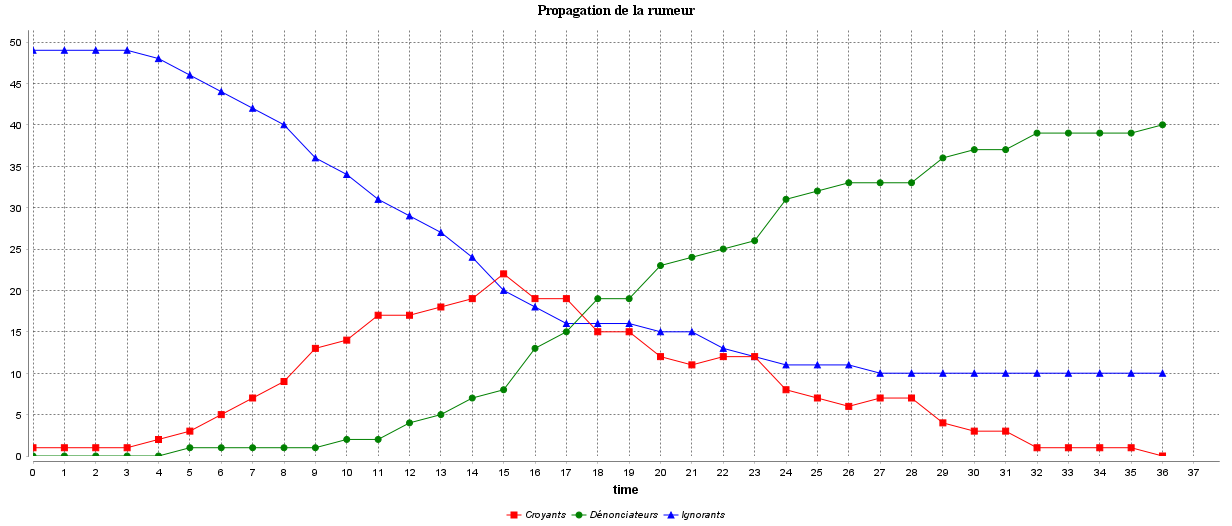
\includegraphics[width=0.95\textwidth]{propagation_rumeur_v2_model_display_Evolution_cycle_36_time_1778255502837.png}
\caption{Évolution des effectifs : croyants, dénonciateurs et ignorants.}
\label{fig:evolution}
\end{figure}

On observe trois phases principales :

\begin{enumerate}
  \item \textbf{Phase d'initiation} : la rumeur démarre avec un seul croyant et une population largement ignorante.
  \item \textbf{Phase de croissance} : le nombre de croyants augmente rapidement, atteint un pic situé autour de 22 individus vers le milieu de la simulation, puis commence à décroître.
  \item \textbf{Phase de correction} : les dénonciateurs deviennent progressivement dominants, ce qui accélère l'effondrement de la croyance.
\end{enumerate}

Cette dynamique est typique d'une rumeur fortement contagieuse mais corrigée par un mécanisme de contre-diffusion. Le graphique montre aussi que la classe des ignorants, initialement majoritaire, se réduit fortement mais ne disparaît pas complètement.

\subsection{Répartition finale}

La Figure~\ref{fig:camembert} représente la structure finale observée au cycle 36.

\begin{figure}[H]
\centering
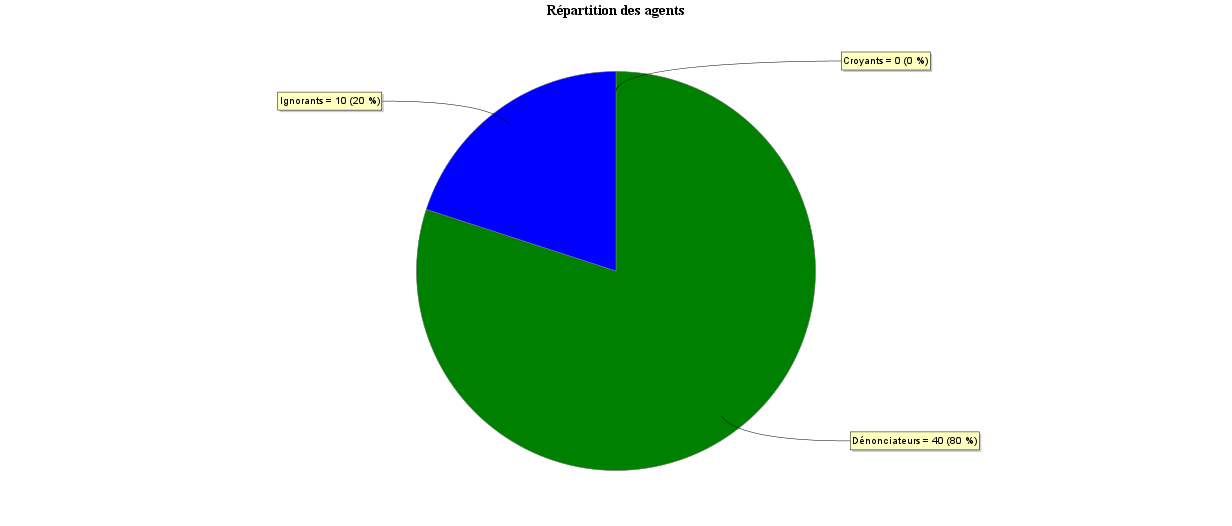
\includegraphics[width=0.80\textwidth]{propagation_rumeur_v2_model_display_Camembert_cycle_36_time_1778255531025.png}
\caption{Répartition finale des agents au cycle 36.}
\label{fig:camembert}
\end{figure}

À ce stade, la simulation indique environ :

\begin{itemize}
  \item 0 croyant, soit 0\% ;
  \item 40 dénonciateurs, soit 80\% ;
  \item 10 ignorants, soit 20\%.
\end{itemize}

Cette distribution confirme que la rumeur a été neutralisée. Le passage massif vers l'état de dénonciateur montre que les mécanismes correctifs ont fini par dominer les mécanismes de propagation.

\subsection{Discussion}

Les résultats obtenus sont cohérents avec le comportement du code GAML. En l'absence d'influenceur et de fact-checker au départ, la diffusion suit d'abord la crédulité moyenne des agents. Ensuite, la propagation s'épuise lorsque les croyants deviennent à leur tour dénonciateurs. Le fait que la population finale se compose majoritairement de dénonciateurs signifie que la rumeur a provoqué un rejet collectif plutôt qu'une adhésion durable.

Le schéma temporel observé est donc :
\[
\text{Ignorants} \to \text{Croyants} \to \text{Dénonciateurs}.
\]
Cette trajectoire suggère un processus de viralité transitoire, suivi d'une régulation par le contre-discours.

\section{Limites du modèle et prolongements possibles}

Le modèle présenté est volontairement simple. Ses limites principales sont :

\begin{itemize}
  \item l'homogénéité de la population, alors que les réseaux sociaux réels sont fortement hétérogènes ;
  \item l'absence de structure explicite de graphe de suiveurs ;
  \item l'approximation moyenne utilisée pour passer du modèle discret au modèle différentiel ;
  \item l'absence de mémoire fine sur les messages successifs et les sources multiples ;
  \item la modélisation simplifiée du fact-checking.
\end{itemize}

Plusieurs prolongements sont possibles :

\begin{itemize}
  \item introduire une classe d'\emph{exposés} pour représenter les agents qui voient la rumeur sans encore y croire ;
  \item intégrer une structure de réseau réelle (petit-monde, échelle libre, communautés fermées) ;
  \item rendre les paramètres dépendants du temps ;
  \item comparer plusieurs scénarios avec et sans influenceur, avec et sans fact-checker ;
  \item calibrer le modèle sur des données empiriques de diffusion en ligne.
\end{itemize}

\section{Conclusion}

Ce travail a proposé une modélisation complète de la propagation d'une rumeur dans un réseau social. À partir du code GAMA fourni, nous avons identifié trois états principaux, construit une approximation compartimentale et écrit un système d'équations différentielles ordinaires décrivant les flux moyens entre ces états. Les simulations montrent une phase de croissance rapide de la croyance, suivie d'une montée forte des dénonciateurs et d'un effondrement de la rumeur. À la fin du cycle observé, la croyance disparaît complètement, tandis que les dénonciateurs dominent la population.

L'étude met en évidence le rôle déterminant du seuil de crédulité, du caractère choquant de la rumeur, et des mécanismes de correction. Elle montre aussi qu'une rumeur peut être fortement virale à court terme tout en étant finalement contenue si les agents correcteurs deviennent suffisamment actifs.

\newpage
\begin{thebibliography}{9}

\bibitem{hethcote2000}
Hethcote, H. W. (2000).
\emph{The Mathematics of Infectious Diseases}.
SIAM Review, 42(4), 599--653.

\bibitem{kermack1927}
Kermack, W. O., \& McKendrick, A. G. (1927).
A contribution to the mathematical theory of epidemics.
\emph{Proceedings of the Royal Society A}, 115(772), 700--721.

\bibitem{taillandier2019}
Taillandier, P., Gaudou, B., Grignard, A., Huynh, Q. N., Marilleau, N., Caillou, P., et al. (2019).
Building, composing and experimenting complex spatial models with the GAMA platform.
\emph{GeoInformatica}, 23(2), 299--322.

\bibitem{gama}
GAMA Platform. Documentation officielle du langage GAML et des expériences de simulation.
\url{https://gama-platform.org/}

\end{thebibliography}

\appendix
\section{Annexe : code GAML utilisé}

Le code complet de la simulation est reproduit ci-dessous.

\begin{small}\begin{verbatim}
/**
 * MODÉLISATION DE LA PROPAGATION D'UNE RUMEUR
 * Version complète corrigée avec graphique + camembert
 */

model propagation_rumeur_v2

global {

    // =========================
    // PARAMÈTRES
    // =========================

    int N <- 50;
    float seuil_moyen <- 2.0;
    float choc_rumeur <- 0.7;

    bool influenceur <- false;
    bool fact_checker <- false;

    // =========================
    // COMPTEURS
    // =========================

    int nb_ignorants <- 0;
    int nb_croyants <- 0;
    int nb_denonciateurs <- 0;

    // =========================
    // SIMULATION
    // =========================

    int current_step <- 0;
    int max_step <- 80;

    int pic_croyants <- 0;
    int temps_pic <- 0;

    // =========================
    // HISTORIQUE
    // =========================

    list<int> hist_croyants <- [];

    // =========================
    // INITIALISATION
    // =========================

    init {

        write "======================================";
        write " PROPAGATION DE RUMEUR - GAMA ";
        write "======================================";

        // Création des utilisateurs
        create utilisateur number: N;

        // Initialisation des agents
        ask utilisateur {

            if (seuil_moyen > 1.0) {

                float alea <- rnd(1.0);

                int s <- int(seuil_moyen + ((alea - 0.5) * 2.0));

                if (s < 1) {
                    s <- 1;
                }

                if (s > 5) {
                    s <- 5;
                }

                seuil <- s;

            } else {

                seuil <- 1;
            }

            influence <- 1;
        }

        // =========================
        // AJOUT INFLUENCEUR
        // =========================

        if (influenceur) {

            ask one_of(utilisateur) {

                influence <- 50;
                seuil <- 1;
            }
        }

        // =========================
        // AJOUT FACT-CHECKER
        // =========================

        if (fact_checker) {

            create utilisateur number: 1 {

                seuil <- 999;
                influence <- 200;
                etat <- "denonciateur";
            }
        }

        // =========================
        // SOURCE INITIALE
        // =========================

        ask one_of(utilisateur) {

            etat <- "croyant";
        }

        // =========================
        // COMPTEURS INITIAUX
        // =========================

        nb_croyants <- length(utilisateur where (each.etat = "croyant"));

        nb_ignorants <- length(utilisateur where (each.etat = "ignorant"));

        nb_denonciateurs <- length(utilisateur where (each.etat = "denonciateur"));

        write "Nombre d'agents : " + string(length(utilisateur));
        write "======================================";
    }

    // =========================
    // BOUCLE PRINCIPALE
    // =========================

    reflex propagation when: (current_step < max_step) and (nb_croyants > 0) {

        current_step <- current_step + 1;

        // Réinitialisation
        ask utilisateur {

            tweets_recus <- 0;
            corrections <- 0;
        }

        // =========================
        // PROPAGATION RUMEUR
        // =========================

        ask utilisateur where (each.etat = "croyant") {

            if (rnd(1.0) < (0.4 * choc_rumeur)) {

                loop i from: 1 to: 3 {

                    utilisateur cible <- one_of(utilisateur);

                    if ((cible != nil) and (cible != self)) {

                        ask cible {

                            tweets_recus <- tweets_recus + 1;
                        }
                    }
                }
            }
        }

        // =========================
        // FACT-CHECKING
        // =========================

        ask utilisateur where (each.etat = "denonciateur") {

            if (rnd(1.0) < 0.4) {

                loop i from: 1 to: 3 {

                    utilisateur cible <- one_of(utilisateur where (each.etat = "croyant"));

                    if (cible != nil) {

                        ask cible {

                            if (rnd(1.0) < min([0.9, influence / 100.0])) {

                                corrections <- corrections + 1;
                            }
                        }
                    }
                }
            }
        }

        // =========================
        // MISE À JOUR ÉTATS
        // =========================

        ask utilisateur {

            // Ignorant -> croyant
            if ((etat = "ignorant") and (tweets_recus >= seuil)) {

                etat <- "croyant";
                temps_etat <- 0;
            }

            // Gestion croyants
            else if (etat = "croyant") {

                temps_etat <- temps_etat + 1;

                // Doute spontané
                if ((temps_etat >= 5) and (rnd(1.0) < 0.25)) {

                    etat <- "denonciateur";
                    temps_etat <- 0;
                }

                // Correction
                else if ((corrections >= 1) and (rnd(1.0) < 0.5)) {

                    etat <- "denonciateur";
                    temps_etat <- 0;
                }
            }
        }

        // =========================
        // MAJ COMPTEURS
        // =========================

        nb_croyants <- length(utilisateur where (each.etat = "croyant"));

        nb_denonciateurs <- length(utilisateur where (each.etat = "denonciateur"));

        nb_ignorants <- length(utilisateur where (each.etat = "ignorant"));

        // Historique
        hist_croyants <- hist_croyants + [nb_croyants];

        // Pic
        if (nb_croyants > pic_croyants) {

            pic_croyants <- nb_croyants;
            temps_pic <- current_step;
        }

        // Affichage console
        if ((current_step mod 10) = 0) {

            write "Step : " + string(current_step)
            + " | Croyants : " + string(nb_croyants)
            + " | Dénonciateurs : " + string(nb_denonciateurs);
        }
    }

    // =========================
    // FIN SIMULATION
    // =========================

    reflex fin when:
        (current_step >= max_step)
        or ((nb_croyants = 0) and (current_step > 10)) {

        write "======================================";
        write " FIN DE LA SIMULATION ";
        write "======================================";

        write "Pic de croyants : " + string(pic_croyants);
        write "Temps du pic : " + string(temps_pic);
        write "Durée : " + string(current_step);

        write "======================================";

        do pause;
    }
}

// =========================
// ESPÈCE UTILISATEUR
// =========================

species utilisateur {

    string etat <- "ignorant";

    int seuil <- 2;

    int influence <- 1;

    int tweets_recus <- 0;

    int corrections <- 0;

    int temps_etat <- 0;
}

// =========================
// EXPÉRIENCE GUI
// =========================

experiment simulation_gui type: gui {

    parameter "Nombre d'agents"
        var: N
        min: 10
        max: 500;

    parameter "Seuil moyen"
        var: seuil_moyen
        min: 1.0
        max: 5.0;

    parameter "Choc rumeur"
        var: choc_rumeur
        min: 0.0
        max: 1.0;

    parameter "Avec influenceur"
        var: influenceur;

    parameter "Avec fact-checker"
        var: fact_checker;

    output {

        // =========================
        // GRAPHIQUE ÉVOLUTION
        // =========================

        display "Evolution" type: 2d {

            chart "Propagation de la rumeur" type: series {

                data "Croyants"
                    value: nb_croyants
                    color: #red;

                data "Dénonciateurs"
                    value: nb_denonciateurs
                    color: #green;

                data "Ignorants"
                    value: nb_ignorants
                    color: #blue;
            }
        }

        // =========================
        // CAMEMBERT
        // =========================

        display "Camembert" type: 2d {

            chart "Répartition des agents" type: pie {

                data "Croyants"
                    value: nb_croyants
                    color: #red;

                data "Dénonciateurs"
                    value: nb_denonciateurs
                    color: #green;

                data "Ignorants"
                    value: nb_ignorants
                    color: #blue;
            }
        }

        // =========================
        // MONITORS
        // =========================

        monitor "Step"
            value: current_step;

        monitor "Croyants"
            value: nb_croyants;

        monitor "Dénonciateurs"
            value: nb_denonciateurs;

        monitor "Ignorants"
            value: nb_ignorants;

        monitor "Pic de croyants"
            value: pic_croyants;

        monitor "Temps du pic"
            value: temps_pic;
    }
}
\end{verbatim}\end{small}

\end{document}
